\documentclass[tikz]{standalone}
\usepackage{xcolor}

\begin{document}
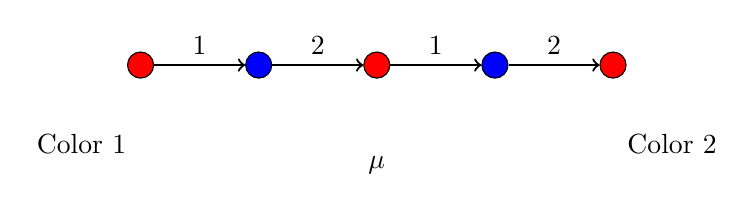
\begin{tikzpicture}[scale=1.5]
    % Define nodes for the sequence
    \node (n1) at (0,0) [circle, draw, fill=red] {};
    \node (n2) at (1,0) [circle, draw, fill=blue] {};
    \node (n3) at (2,0) [circle, draw, fill=red] {};
    \node (n4) at (3,0) [circle, draw, fill=blue] {};
    \node (n5) at (4,0) [circle, draw, fill=red] {};

    % Draw paths between nodes
    \draw[thick, ->] (n1) -- node[midway, above] {1} (n2);
    \draw[thick, ->] (n2) -- node[midway, above] {2} (n3);
    \draw[thick, ->] (n3) -- node[midway, above] {1} (n4);
    \draw[thick, ->] (n4) -- node[midway, above] {2} (n5);

    % Add labels for colors
    \node at (-0.5,-0.5) [below] {Color 1};
    \node at (4.5,-0.5) [below] {Color 2};

    % Add labels for the sequence
    \node at (2,-1) [above] {\(\bm{\mu}\)};
\end{tikzpicture}
\end{document}